% ResearchPhO question paper: How does disorder enter a model, a Hall current and a pump?
% Compile twice with pdflatex. Questions only: no answers, no research notes.
\documentclass[11pt,a4paper]{article}
\usepackage[T1]{fontenc}
\usepackage[utf8]{inputenc}
\usepackage{fix-cm}
\usepackage[scaled=0.96]{helvet}
\renewcommand{\familydefault}{\sfdefault}
\usepackage{amsmath,amssymb,mathtools}
\usepackage{newtxmath}
\usepackage{bm,dsfont}
\usepackage[margin=20mm,top=35mm,bottom=20mm,headheight=57pt,headsep=10mm]{geometry}
\usepackage{microtype,booktabs,array,tabularx,enumitem,needspace}
\usepackage[most]{tcolorbox}
\usepackage{fancyhdr,xcolor}
\usepackage{tikz}
\usetikzlibrary{arrows.meta,calc,positioning,shapes.geometric,decorations.pathreplacing,decorations.pathmorphing,decorations.markings}
\usepackage{pgfplots}
\pgfplotsset{compat=1.18}
\usepackage[hidelinks,pdfencoding=auto,psdextra]{hyperref}
\hypersetup{pdftitle={ResearchPhO: How does disorder enter a model, a Hall current and a pump? - Theory Questions},pdfsubject={ResearchPhO: research-based exam in IPhO/APhO format}}
\definecolor{ink}{HTML}{172A3A}
\definecolor{rulegray}{HTML}{5E6670}
\definecolor{colA}{HTML}{D9822B}
\definecolor{colB}{HTML}{3C78B4}
\definecolor{colG}{HTML}{1B6B4B}
\definecolor{colR}{HTML}{A42B32}
\setlength{\parindent}{0pt}
\setlength{\parskip}{5.4pt}
\setlength{\emergencystretch}{2em}
\setlength{\abovedisplayskip}{6pt}
\setlength{\belowdisplayskip}{6pt}
\raggedbottom
% ---------------- page codes ----------------
\newcounter{problemno}
\newcounter{figc}
\renewcommand{\thefigc}{\arabic{problemno}.\arabic{figc}}
\newcommand{\pagecode}{G}
\renewcommand{\thepage}{\pagecode-\arabic{page}}
\pagestyle{fancy}
\fancyhf{}
\fancyhead[L]{\begin{minipage}[b]{0.73\textwidth}\textbf{\large Theory}\\[-1pt]{\small ResearchPhO \enspace|\enspace Questions}\\[-1pt]{\footnotesize English}\end{minipage}}
\fancyhead[R]{\fontsize{29}{31}\selectfont\bfseries \thepage}
\renewcommand{\headrulewidth}{0.9pt}
\fancyfoot[L]{\footnotesize ResearchPhO --- a research-based exam in IPhO/APhO format; not an official olympiad paper}
% ---------------- notation ----------------
\newcommand{\ket}[1]{\lvert #1\rangle}
\newcommand{\bra}[1]{\langle #1\rvert}
\newcommand{\Tr}{\operatorname{Tr}}
\newcommand{\dd}{\mathrm d}
\newcommand{\id}{\mathds 1}
\newcommand{\hc}{\mathrm{h.c.}}
\newcommand{\avg}[1]{\overline{#1}}
\newcommand{\Var}{\operatorname{Var}}
\newcommand{\Cov}{\operatorname{Cov}}
\newcommand{\eF}{\varepsilon_{\rm F}}
% ---------------- structure ----------------
\newcommand{\problem}[3]{\clearpage\setcounter{problemno}{#1}\renewcommand{\pagecode}{T#1}\setcounter{page}{1}\setcounter{figc}{0}{\LARGE\bfseries\color{ink}Problem #1: #2}\hfill{\large\bfseries(#3 points)}\par\medskip}
\newcommand{\parttitle}[3]{\par\Needspace{8\baselineskip}\vspace{6pt}{\large\bfseries\color{ink}Part #1. #2\hfill\normalsize(#3 points)}\par\vspace{2pt}}
\newcommand{\smallheading}[1]{\par\Needspace{6\baselineskip}\medskip\textbf{#1}\par}
\newcommand{\question}[3]{\begin{tcolorbox}[enhanced,colback=white,colframe=rulegray,boxrule=0.5pt,arc=0pt,left=7pt,right=7pt,top=7pt,bottom=7pt,before skip=9pt,after skip=9pt]\begin{tabularx}{\linewidth}{@{}>{\bfseries}p{10mm}X>{\raggedleft\arraybackslash}p{13mm}@{}}#1&#3&\textbf{#2 pt}\end{tabularx}\end{tcolorbox}}
\newcommand{\hint}[1]{\par{\small\textbf{Hint.} #1}\par}
\newenvironment{figpanel}[1]{\refstepcounter{figc}\gdef\figtitle{#1}\par\medskip\noindent\begin{minipage}{\linewidth}\centering}{\end{minipage}\par\medskip}
\newcommand{\figtext}[1]{\par\smallskip{\raggedright\small\textbf{Figure \thefigc.} \figtitle. #1\par}}
\newcolumntype{Y}{>{\raggedright\arraybackslash}X}
\tikzset{>={Stealth[length=2.2mm]},
  atom/.style={circle,draw=ink,fill=white,inner sep=0pt,minimum size=5.2mm,font=\scriptsize},
  ghost/.style={circle,draw=black!30,dashed,inner sep=0pt,minimum size=5.2mm},
  imp/.style={star,star points=5,star point ratio=2.2,fill=colR,draw=colR,inner sep=0pt,minimum size=3.2mm}}
\pgfplotsset{mbaxis/.style={width=7.6cm,height=5.4cm,tick label style={font=\scriptsize},label style={font=\small},axis line style={rulegray},tick style={rulegray},legend style={font=\scriptsize,draw=none,fill=none}}}
\begin{document}

{\LARGE\bfseries\color{ink}How does disorder enter a model, a Hall current and a pump?}\par
{\large ResearchPhO --- Theoretical examination \hfill \textbf{30 points}}

\smallheading{General instructions}
\begin{enumerate}[leftmargin=7mm,itemsep=3pt]
\item The theoretical examination lasts 5 hours. It has three problems; each problem is worth 10 points.
\item You may use a non-programmable scientific calculator. No other aids are allowed.
\item Write your answers on plain sheets. Label each answer with its question (for example 1.A.1) and box each final result. Derivations count: show the steps you want graded.
\item Write on the front side of the sheets only. Use as few words as possible: express yourself with equations, numbers, symbols and diagrams.
\item The problems are independent and can be solved in any order. Within a problem, later questions can often be answered without the earlier results.
\item Each problem states its own conventions. A bar over a quantity, $\avg{O}$, always means an average: over disorder configurations, over the noise, or over the regions of a sample, as stated.
\end{enumerate}

\smallheading{Problems}
{\small\begin{tabularx}{\textwidth}{@{}p{18mm}Y r@{}}\toprule
Problem&Title and parts&Points\\\midrule
1&From a dirty crystal to a random Hamiltonian. A: from an impurity to lattice parameters; B: displaced atoms; C: from correlations to rates; D: which random term first?&10.0\\
2&Impurities and the second-order Hall current. A: three sources of a Hall current; B: a dipole of curvature; C: collisions enter at the same order; D: one broadening, many ensembles&10.0\\
3&Disorder in a two-cycle quantum pump. A: topology from disorder in a dimer chain; B: counting the pumped charge; C: what a random potential does to the flavors; D: domains in a long disordered chain&10.0\\\midrule
&&\textbf{30.0}\\\bottomrule
\end{tabularx}}

%%%%%%%%%%%%%%%%%%%%%%%%%%%%%%%%%%%%%%%%%%%%%%%%%%%%%%%%%%%%%%%%%%%%%%%%%%%%%%%%%%%%%%%%%%%%%%%%
\problem{1}{From a dirty crystal to a random Hamiltonian}{10.0}

No crystal is perfect. Foreign atoms replace host atoms, some atoms are missing, atoms sit slightly off their ideal positions, charges are trapped in the substrate, the lattice vibrates and gate voltages fluctuate. An experiment controls only the average composition and structure of a sample; an electron moves in one particular arrangement of all these imperfections. A theory of a measured response must therefore decide which imperfections to keep and how to represent them.

A model of static disorder (a \emph{disorder model}) has two ingredients. For every arrangement $\mathcal C$ of the imperfections (a \emph{disorder configuration}) it gives a Hamiltonian $H_{\mathcal C}$, and it gives the probability $P[\mathcal C]$ of each arrangement. A quantity $O$ is computed first in one configuration and then averaged over configurations (the \emph{disorder average}):
\[
\avg O=\sum_{\mathcal C}P[\mathcal C]\,O_{\mathcal C}.
\]
The simplest example is a chain of atoms with one orbital per atom and random orbital energies (the \emph{Anderson model}),
\[
H_{\mathcal C}=-J\sum_j\big(c_{j+1}^\dagger c_j+c_j^\dagger c_{j+1}\big)+\sum_j\epsilon_j n_j ,
\]
where $c_j^\dagger$ creates an electron in the orbital of atom $j$, $n_j=c_j^\dagger c_j$, $J>0$ is the hopping amplitude, and the on-site energies $\epsilon_j$ are random numbers. For one electron, $H_{\mathcal C}$ is the matrix with diagonal elements $\epsilon_j$ and elements $-J$ between neighbouring atoms.

Without disorder, a response formula contains factors $1/(E-E_{\bm k})$, where $E_{\bm k}$ is the energy of a state of momentum $\bm k$. The simplest way to include disorder replaces them by $1/(E-E_{\bm k}+i\Gamma)$: every level becomes a Lorentzian of half-width $\Gamma$ (the \emph{broadening}), and an electron leaves its state at the rate $1/\tau=2\Gamma/\hbar$. This problem builds disorder models from microscopic ingredients and turns them into such rates. It asks: \emph{which random terms must a model of a real material contain first, and how do they become the scattering rate and the level broadening that response theories use?}

\begin{figpanel}{Orbitals and two impurity positions}\label{fig:orbitals}
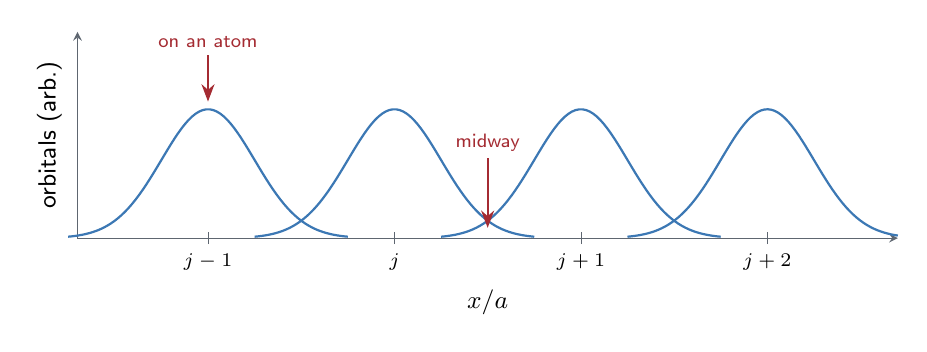
\begin{tikzpicture}
\begin{axis}[mbaxis,width=12cm,height=4.2cm,xmin=-1.7,xmax=2.7,ymin=0,ymax=1.6,
  xlabel={$x/a$},ylabel={orbitals (arb.)},xtick={-1,0,1,2},xticklabels={$j-1$,$j$,$j+1$,$j+2$},ytick=\empty,axis x line=bottom,axis y line=left,clip=false]
\addplot[colB,thick,domain=-1.75:-0.25,samples=80] {exp(-8*(x+1)^2)};
\addplot[colB,thick,domain=-0.75:0.75,samples=80] {exp(-8*(x)^2)};
\addplot[colB,thick,domain=0.25:1.75,samples=80] {exp(-8*(x-1)^2)};
\addplot[colB,thick,domain=1.25:2.7,samples=80] {exp(-8*(x-2)^2)};
\draw[colR,thick,->] (axis cs:-1,1.42) -- (axis cs:-1,1.06);
\node[font=\scriptsize,text=colR,anchor=south] at (axis cs:-1,1.40) {on an atom};
\draw[colR,thick,->] (axis cs:0.5,0.62) -- (axis cs:0.5,0.08);
\node[font=\scriptsize,text=colR,anchor=south] at (axis cs:0.5,0.60) {midway};
\end{axis}
\end{tikzpicture}
\figtext{Gaussian orbitals with $b=a/4$, centred on the atoms. A point-like impurity (red arrow) can sit on an atom or midway between two atoms; one example of each kind is drawn.}
\end{figpanel}

\smallheading{Useful information}
\begin{itemize}[leftmargin=6mm,itemsep=2pt,topsep=2pt]
\item For random variables $x,y$: $\Cov(x,y)=\avg{xy}-\avg x\,\avg y$; $\Var x=\Cov(x,x)$; the correlation coefficient is $\Cov(x,y)/\sqrt{\Var x\,\Var y}$; the third cumulant is $\kappa_3=\avg{(x-\avg x)^3}$. For independent $x,y$: $\avg{xy}=\avg x\,\avg y$, and the variance of a sum of independent variables is the sum of their variances.
\item A variable distributed uniformly on $[-W/2,W/2]$ has mean $0$, variance $W^2/12$ and $\kappa_3=0$.
\item Fermi's golden rule: a perturbation $V$ takes the state $\ket i$ into a continuum of states $\ket f$ at the rate $\frac{2\pi}{\hbar}\sum_f|\langle f|V|i\rangle|^2\delta(E_f-E_i)$.
\item On a ring of $L$ sites, with $k=2\pi m/L$ and $k'=2\pi m'/L$ ($m,m'$ integers): $\sum_{j=1}^{L}e^{i(k-k')j}=L\,\delta_{kk'}$.
\item $\int_{-\infty}^{\infty}e^{-\alpha x^2/2}\dd x=\sqrt{2\pi/\alpha}$ and $\int_{-\infty}^{\infty}x^2e^{-\alpha x^2/2}\dd x=\sqrt{2\pi/\alpha}\,/\alpha$ for $\alpha>0$.
\item Classical noise $\eta(t)$ with zero mean has the correlation function $\avg{\eta(t)\eta(0)}$ (an average over the noise) and the spectrum $S(\omega)=\int_{-\infty}^{\infty}e^{i\omega t}\,\avg{\eta(t)\eta(0)}\,\dd t$. A weak perturbation $\eta(t)A$, with $A$ an operator, causes transitions $\ket0\to\ket1$ between eigenstates with $E_1-E_0=\hbar\omega_0$ at the rate $r_{10}=|\langle1|A|0\rangle|^2S(\omega_0)/\hbar^2$.
\item For a zero-mean random $x$ with small variance and a smooth function $F$, to leading order: $\avg{F(x)}\approx F(0)+\tfrac12F''(0)\avg{x^2}$ and $\Var F(x)\approx F'(0)^2\avg{x^2}$.
\item $\hbar=6.582\times10^{-13}$ meV\,s.
\end{itemize}

\parttitle{A}{From an impurity to lattice parameters}{2.4}
Atoms sit at $x=ja$. Atom $j$ carries the orbital $\varphi_j(x)=(\pi b^2)^{-1/4}\exp[-(x-ja)^2/(2b^2)]$, whose size is set by $b<a$ (Fig.~\ref{fig:orbitals}). Treat these orbitals as orthonormal, neglecting their overlap; this is a model, in which the small numbers below are only estimates, but small numbers stay small. A short-range impurity at position $x_0$ has the potential $v(x)=u_0\,\delta(x-x_0)$. It changes the one-electron matrix elements by
\[
\delta h_{ij}=\int\varphi_i(x)\,v(x)\,\varphi_j(x)\,\dd x .
\]
$\delta h_{jj}$ changes the energy of orbital $j$ (an on-site term); $\delta h_{j,j+1}$ changes the hopping between atoms $j$ and $j+1$ (a bond term).

\question{A.1}{1.2}{\textbf{(a)} Find $\delta h_{jj}$, $\delta h_{j+1,j+1}$ and $\delta h_{j,j+1}$ for an impurity on atom $j$ ($x_0=ja$) and for an impurity midway between atoms $j$ and $j+1$ ($x_0=(j+\frac12)a$).\par
\textbf{(b)} Evaluate $|\delta h_{j,j+1}/\delta h_{jj}|$ in both cases for $a/b=4$. For which kind of impurity is a model with random on-site energies only (the Anderson model) adequate?\par
\textbf{(c)} Show that the matrix $\delta h_{ij}$ produced by one impurity is the product of a single vector with itself. Impurities with random strengths $u_0$ sit at random positions $x_0$. What does this product form imply for the statistical relation between the on-site and the bond terms produced by the same impurity?}

Two distributions of the on-site energies are compared. \emph{Model 1:} the $\epsilon_j$ are independent and uniform on $[-W/2,W/2]$. \emph{Model 2 (binary alloy):} each atom is, independently, a host atom with $\epsilon_j=0$ (probability $1-f_{\rm s}$) or a substitute atom with $\epsilon_j=\epsilon_{\rm s}>0$ (probability $f_{\rm s}$, with $0<f_{\rm s}<1$).

\question{A.2}{1.2}{\textbf{(a)} For model 2, find the mean $\avg{\epsilon_j}$, the variance $\kappa_2$ and the third cumulant $\kappa_3$. The mean does not appear among the random terms of the disorder model: which part of the Hamiltonian absorbs it?\par
\textbf{(b)} Choose $\epsilon_{\rm s}$ so that model 2 has the same variance as model 1. For $f_{\rm s}=0.1$, find $\epsilon_{\rm s}/W$ and $\kappa_3/W^3$. Find the value of $f_{\rm s}$ in $(0,1)$ for which $\kappa_3=0$.\par
\textbf{(c)} A calculation to second order in the random potential depends on $\kappa_2$ only. Explain why the two models with equal $\kappa_2$ can still give different results for a quantity that first appears at third order in the random potential. What happens to $\kappa_2$ and $\kappa_3$ if every substitute atom is replaced by one with $\epsilon_j=-\epsilon_{\rm s}$?}

\parttitle{B}{Displaced atoms}{2.2}
Atoms in an array, for instance atoms held by focused laser beams (optical tweezers) in a quantum simulator, sit at $x_j=ja+u_j$ (Fig.~\ref{fig:displaced}). The displacements $u_j$ are independent, with zero mean and variance $\sigma_u^2$, $\sigma_u\ll a$. Bond $j$ joins atoms $j$ and $j+1$; its length is $d_j=x_{j+1}-x_j$ and its hopping is $J_j=J(d_j)$, a smooth function of the distance. Write $\delta J_j=J_j-J(a)$ and define the spectrum of the bond disorder, with a dimensionless wavenumber $q$, as
\[
K_J(q)=\sum_{n=-\infty}^{\infty}e^{-iqn}\,\Cov(\delta J_j,\delta J_{j+n}).
\]

\begin{figpanel}{Displaced atoms}\label{fig:displaced}
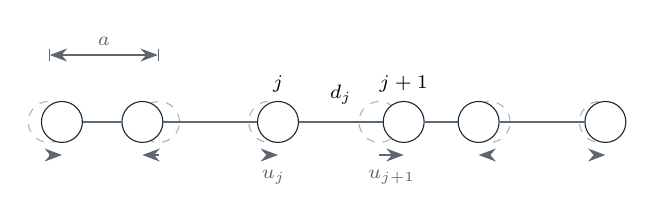
\begin{tikzpicture}[x=14mm,y=10mm]
\foreach \x in {0,...,5}{\node[ghost] at (\x,0) {};}
\foreach \x/\u in {0/0.12,1/-0.15,2/0.08,3/0.22,4/-0.1,5/0.05}{\node[atom] (a\x) at (\x+\u,0) {};}
\foreach \x/\u in {0/0.12,1/-0.15,2/0.08,3/0.22,4/-0.1,5/0.05}{\draw[rulegray,->] (\x,-0.42)--(\x+\u,-0.42);}
\node[font=\scriptsize,text=rulegray] at (2.04,-0.7) {$u_j$};
\node[font=\scriptsize,text=rulegray] at (3.11,-0.7) {$u_{j+1}$};
\foreach \x [evaluate=\x as \y using int(\x+1)] in {0,...,4}{\draw[ink!70,line width=1pt] (a\x)--(a\y);}
\node[font=\scriptsize,above=3pt] at ($(a2)!0.5!(a3)$) {$d_j$};
\node[font=\scriptsize] at (2.08,0.48) {$j$};
\node[font=\scriptsize] at (3.22,0.48) {$j+1$};
\draw[|<->|,rulegray] (0,0.85)--(1,0.85) node[midway,above,font=\scriptsize]{$a$};
\end{tikzpicture}
\figtext{Dashed circles: ideal positions $ja$. Solid circles: actual positions $ja+u_j$; grey arrows: the displacements (exaggerated). Bond $j$ has length $d_j=a+u_{j+1}-u_j$.}
\end{figpanel}

\question{B.1}{1.2}{\textbf{(a)} To first order in the displacements, find $\delta J_j$, $\Var(\delta J_j)$, $\Cov(\delta J_j,\delta J_{j+1})$ and $\Cov(\delta J_j,\delta J_{j+n})$ for $n\ge2$.\par
\textbf{(b)} Find $K_J(q)$ and its value at $q=0$. Show that the variance of $\sum_{j=1}^{M}\delta J_j$ does not grow with $M$, and explain this physically.\par
\textbf{(c)} A simpler model draws every $J_j$ independently, with the same variance as in (a). Find its $K_J(q)$. Compare, in the two models, how the fluctuation of the \emph{average} hopping of a stretch of $M$ bonds decreases with $M$.}

For atoms excited to high-lying (Rydberg) states, the hopping of an excitation between two atoms a distance $r$ apart is $J=C_3(1-3\cos^2\theta)/(2r^3)$, where $\theta$ is the angle between the line joining the atoms and an applied magnetic field; here $\theta=90^\circ$, so $J(r)=C_3/(2r^3)$. The interaction energy between two neighbouring excitations is $V_6(r)=C_6/r^6$. $C_3,C_6>0$. Both depend on the same bond length: $J_j=J(d_j)$, $V_{6,j}=V_6(d_j)$.

\question{B.2}{1.0}{\textbf{(a)} To first order, express $\delta J_j/J(a)$ and $\delta V_{6,j}/V_6(a)$ through $u_{j+1}-u_j$. Find the correlation coefficient of $\delta J_j$ and $\delta V_{6,j}$, and the root-mean-square (rms) values of $\delta J_j/J(a)$ and $\delta V_{6,j}/V_6(a)$ for $\sigma_u=0.03a$.\par
\textbf{(b)} To second order, find $\avg{J_j}/J(a)-1$ and $\avg{V_{6,j}}/V_6(a)-1$, and evaluate them for $\sigma_u=0.03a$.\par
\textbf{(c)} A simulation draws $J_j$ and $V_{6,j}$ independently, each with mean $J(a)$ or $V_6(a)$ and with the variance of (a). State two features of the real ensemble that this simulation misses.}

\parttitle{C}{From correlations to rates}{3.2}
Take model 1 on a ring of $L$ sites with lattice constant $a$. Without disorder the eigenstates are the plane waves $\ket k=L^{-1/2}\sum_je^{ikj}\ket j$, $k=2\pi m/L$, with energies $E_k=-2J\cos k$ and group velocities $v_k=(2Ja/\hbar)\sin k$. The number of states per unit energy and per site, counting both directions of motion, is $\nu(E)=1/\big(\pi\sqrt{4J^2-E^2}\big)$. The random potential $\sum_j\epsilon_jn_j$ has matrix elements $V_{k'k}$ between plane waves. The golden-rule rate at which an electron leaves the state $\ket k$ defines its \emph{single-particle lifetime} $\tau$; the broadening of the level is $\Gamma=\hbar/(2\tau)$.

\question{C.1}{1.3}{\textbf{(a)} Show that $\avg{|V_{k'k}|^2}=W^2/(12L)$ for $k'\neq k$.\par
\textbf{(b)} Find $1/\tau$ for a state at energy $E=J$ (that is, $k=2\pi/3$), the broadening $\Gamma$ and the mean free path $\ell=|v_k|\tau$. Evaluate $\Gamma/J$ and $\ell/a$ for $W=J$.\par
\textbf{(c)} A calculation that keeps the interference of multiply scattered waves shows that, for weak disorder, every eigenstate of the chain is localized: its amplitude decays as $e^{-|x|/\xi}$, with $\xi=24(4J^2-E^2)a/W^2$ away from the centre and the edges of the band. Find $\xi/\ell$ at $E=J$. For a wire of length $L_{\rm w}\gg\xi$ the zero-temperature conductance is of order $(e^2/h)e^{-2L_{\rm w}/\xi}$, while an estimate that uses only $\tau$ (a Drude estimate) gives a conductance of order $(e^2/h)\,\ell/L_{\rm w}$. Evaluate both for $L_{\rm w}=1000a$ and $W=J$. Which comparison of lengths decides whether the $\tau$-based estimate is meaningful? At finite temperature, inelastic collisions with phonons or other electrons destroy the phase memory of an electron after a distance $L_\varphi$ (the \emph{dephasing length}); state the condition on $L_\varphi$ under which a $\tau$-based description becomes meaningful again.}

In a two-dimensional electron gas with a parabolic band and Fermi wavenumber $k_{\rm F}$, a random potential $U(\bm r)$ has the correlation $\avg{U(\bm r)U(\bm 0)}=U_0^2e^{-r^2/(2\lambda^2)}$, whose Fourier transform is $K_U(Q)\propto e^{-Q^2\lambda^2/2}$; $\lambda$ is the correlation length. Elastic scattering by an angle $\theta$ on the Fermi circle transfers the wavenumber $Q=2k_{\rm F}|\sin(\theta/2)|$ (Fig.~\ref{fig:fermicircle}). In the golden-rule approximation,
\[
\frac1{\tau_q}=B\int_{-\pi}^{\pi}K_U\big(Q(\theta)\big)\,\dd\theta,\qquad
\frac1{\tau_{\rm tr}}=B\int_{-\pi}^{\pi}K_U\big(Q(\theta)\big)(1-\cos\theta)\,\dd\theta,
\]
where $B$ is a constant. $\tau_q$ is the single-particle lifetime (defined as above); $\tau_{\rm tr}$, the \emph{transport lifetime}, is the time over which the direction of the current is lost. The electron mobility is proportional to $\tau_{\rm tr}$.

\begin{figpanel}{Elastic scattering on the Fermi circle}\label{fig:fermicircle}
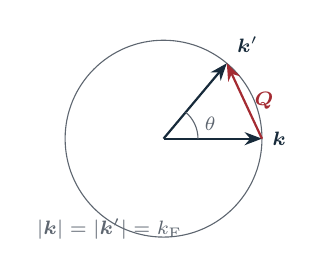
\begin{tikzpicture}[scale=1.25]
\draw[rulegray] (0,0) circle (1);
\draw[->,ink,thick] (0,0)--(1,0) node[right,font=\scriptsize]{$\bm k$};
\draw[->,ink,thick] (0,0)--({cos(50)},{sin(50)}) node[above right,font=\scriptsize]{$\bm k'$};
\draw[->,colR,thick] (1,0)--({cos(50)},{sin(50)}) node[midway,right,font=\scriptsize]{$\bm Q$};
\draw[rulegray] (0.35,0) arc (0:50:0.35) node[midway,right,font=\scriptsize]{$\theta$};
\node[font=\scriptsize,text=rulegray] at (-0.55,-0.92) {$|\bm k|=|\bm k'|=k_{\rm F}$};
\end{tikzpicture}
\figtext{An electron with wavevector $\bm k$ is scattered elastically to $\bm k'$ on the same circle; the transferred wavevector is $\bm Q=\bm k'-\bm k$.}
\end{figpanel}

\question{C.2}{1.1}{\textbf{(a)} Find $\tau_{\rm tr}/\tau_q$ for $\lambda\to0$.\par
\textbf{(b)} For $k_{\rm F}\lambda\gg1$, show that $\tau_{\rm tr}/\tau_q\approx2(k_{\rm F}\lambda)^2$.\par
\textbf{(c)} Two samples have the same broadening $\Gamma=\hbar/(2\tau_q)$; one has short-range disorder ($\lambda\to0$), the other smooth disorder with $k_{\rm F}\lambda=3$. Using (b), estimate the mobility of the smooth sample divided by that of the short-range sample. What does adding $\Gamma$ to the energies in a clean response formula capture, and what does it miss?}

\question{C.3}{0.8}{\textbf{(a)} Two sites with $h=\begin{pmatrix}\epsilon_1&-J\\-J&\epsilon_2\end{pmatrix}$; the electron starts on site 1 at $t=0$. Find the probability $P_2(t)$ of finding it on site 2. Does static disorder make the electron leave site 1 irreversibly?\par
\textbf{(b)} The golden rule in C.1 treats the final states as a continuum. On a ring of $L$ sites the levels are discrete; the time needed to resolve them is the \emph{Heisenberg time} $t_{\rm H}=2\pi\hbar L\nu(E)$. State a condition comparing $\tau$ with $t_{\rm H}$, and a second condition comparing $\Gamma$ with the band width $4J$, under which a decay of $\ket k$ at the rate $1/\tau$ can be observed. Evaluate $t_{\rm H}$ for $L=1000$ and $E=J$ in units of $\hbar/J$, and compare it with $\tau$ at $W=J$.}

\parttitle{D}{Which random term first?}{2.2}
Two eigenstates $\ket0$ and $\ket1$, split by $\hbar\omega_0=10$ meV, determine a measured quantity (for example, the two bands that come closest in energy at the momentum where a response is concentrated). A fluctuating perturbation $\eta(t)A$ acts on them; $\eta$ is classical noise with $\avg{\eta(t)\eta(0)}=\sigma_\eta^2e^{-|t|/\tau_{\rm c}}$, where $\tau_{\rm c}$ is its correlation time, so that $S(\omega)=2\sigma_\eta^2\tau_{\rm c}/(1+\omega^2\tau_{\rm c}^2)$. Take $|\langle1|A|0\rangle|\,\sigma_\eta=0.1$ meV. The rate formula describes observation times longer than $\tau_{\rm c}$ and $1/\omega_0$.

\question{D.1}{1.0}{\textbf{(a)} At fixed $\sigma_\eta$, find the correlation time $\tau_{\rm c}$ that maximizes the transition rate $r_{10}$, and the maximal rate in s$^{-1}$.\par
\textbf{(b)} Find $r_{10}$ for $\tau_{\rm c}=1$ ns and for $\tau_{\rm c}=1$ fs at the same $\sigma_\eta$.\par
\textbf{(c)} Evaluate $r_{10}t_{\rm obs}$ for the three cases of (a) and (b), for an ultrafast optical measurement ($t_{\rm obs}=1$ ps) and for a slow pumping experiment ($t_{\rm obs}=10\ \mu$s). For which case is a rate not the right description at $t_{\rm obs}=1$ ps?\par
\textbf{(d)} What does the formula give for static disorder ($\tau_{\rm c}\to\infty$)? How must static disorder be treated instead?\par
\textbf{(e)} Find $r_{10}$ if $A=\hat N$, the total number of electrons of an isolated sample, and $\ket0,\ket1$ are eigenstates of a Hamiltonian that conserves $\hat N$.}

A response coefficient $\chi$ depends on the local chemical potential near a band feature as
\[
\chi(\mu)=\chi_0\frac{\Lambda^2}{(\mu-\mu_0)^2+\Lambda^2},\qquad \Lambda=10\ \text{meV}.
\]
Trapped charges make the local chemical potential $\mu+\delta\mu(\bm r)$ vary in space (\emph{charge puddles}), with zero-mean Gaussian $\delta\mu$ of rms $\sigma_\mu=3$ meV. Assume that each puddle responds locally to the same applied field, that the measured $\chi$ is the average over $N_{\rm p}\gg1$ independent puddles, and that the puddles are much smaller than the sample.

\question{D.2}{0.8}{\textbf{(a)} To leading order in $\sigma_\mu/\Lambda$: at $\mu=\mu_0$, find the fractional shift of the averaged $\chi$; at $\mu=\mu_0+\Lambda$, find the rms puddle-to-puddle variation of the local $\chi$, relative to $\chi(\mu_0+\Lambda)$.\par
\textbf{(b)} Which of the two effects in (a) survives in the measured $\chi$ when $N_{\rm p}\to\infty$, and how does the other scale with $N_{\rm p}$?\par
\textbf{(c)} State two conditions under which this estimate fails.}

\question{D.3}{0.4}{Using the results of this problem, list three tests that decide whether a random term must enter the model of a given measurement: one on how the term couples to the relevant states, one on time scales, and one on its effect on the measured quantity. For each test, state what is compared with what.}

%%%%%%%%%%%%%%%%%%%%%%%%%%%%%%%%%%%%%%%%%%%%%%%%%%%%%%%%%%%%%%%%%%%%%%%%%%%%%%%%%%%%%%%%%%%%%%%%
\problem{2}{Impurities and the second-order Hall current}{10.0}

An electric field $\bm E$ in a conductor can drive a current perpendicular to $\bm E$ (a \emph{Hall current}) even without a magnetic field. In a magnetic conductor this \emph{anomalous Hall effect} has three microscopic sources (Fig.~\ref{fig:mechanisms}). (1) Band geometry: an electron wave packet acquires a velocity perpendicular to the applied force (the \emph{anomalous velocity}), set by a property of the band called the Berry curvature $\Omega(\bm k)$ (the \emph{intrinsic} contribution). (2) In each collision with an impurity, the centre of the wave packet jumps sideways by a small distance $\delta\bm r$ (\emph{side jump}). (3) Collisions are asymmetric: an electron is scattered more often to one side than to the other (\emph{skew scattering}). Sources (2) and (3) exist only because of disorder.

A crystal that is symmetric under time reversal (no magnetic order, no magnetic field) has no Hall current linear in $\bm E$. A Hall current proportional to $E^2$ is still allowed if the crystal lacks inversion symmetry (the \emph{nonlinear Hall effect}). It is measured by passing an alternating current of low frequency $\omega$ along $x$ and detecting a transverse voltage at frequency $2\omega$. This second-order current was first explained by band geometry alone.

\begin{figpanel}{Three sources of a Hall current}\label{fig:mechanisms}
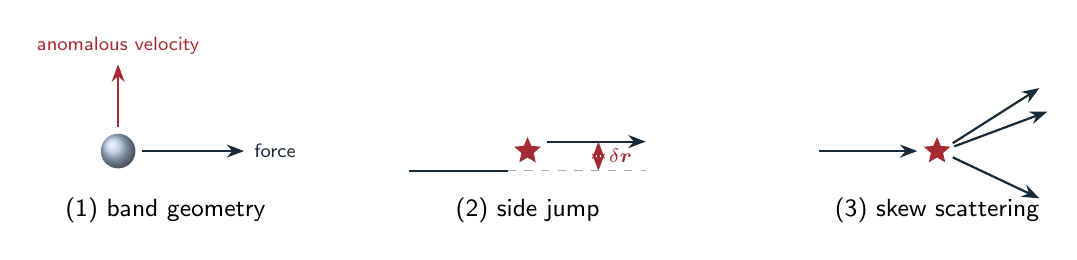
\begin{tikzpicture}[x=10mm,y=10mm]
\begin{scope}
\shade[ball color=colB!40] (0,0) circle (0.22);
\draw[->,ink,thick] (0.3,0)--(1.6,0) node[right,font=\scriptsize]{force};
\draw[->,colR,thick] (0,0.3)--(0,1.1) node[above,font=\scriptsize]{anomalous velocity};
\node[font=\small] at (0.6,-0.75) {(1) band geometry};
\end{scope}
\begin{scope}[xshift=52mm]
\node[imp] (i) at (0,0) {};
\draw[ink,thick] (-1.5,-0.25)--(-0.25,-0.25);
\draw[ink,thick,->] (0.25,0.12)--(1.5,0.12);
\draw[colR,thick,<->] (0.9,-0.25)--(0.9,0.12) node[midway,right,font=\scriptsize]{$\delta\bm r$};
\draw[ink!40,dashed] (-0.25,-0.25)--(1.5,-0.25);
\node[font=\small] at (0,-0.75) {(2) side jump};
\end{scope}
\begin{scope}[xshift=104mm]
\node[imp] (j) at (0,0) {};
\draw[ink,thick,->] (-1.5,0)--(-0.25,0);
\draw[ink,thick,->] (0.2,0.1)--(1.3,0.8);
\draw[ink,thick,->] (0.22,0.06)--(1.4,0.5);
\draw[ink,thick,->] (0.2,-0.08)--(1.3,-0.6);
\node[font=\small] at (0,-0.75) {(3) skew scattering};
\end{scope}
\end{tikzpicture}
\figtext{(1) For one sign of $\Omega$, a wave packet moves partly perpendicular to the force. (2) A collision displaces the packet sideways by $\delta\bm r$; the dashed line continues the incoming path without the jump. (3) An impurity scatters more electrons to the left of the incoming direction (two arrows) than to the right (one arrow). Red stars: impurities.}
\end{figpanel}

\smallheading{Model and conventions}
Electrons with charge $-e$ ($e>0$) move in two dimensions. Near one point of the Brillouin zone they are described by the $2\times2$ Hamiltonian
\[
H(\bm k)=v_tk_x\,\id+v\,(k_xs_x+k_ys_y)+m\,s_z,
\]
a \emph{tilted massive Dirac cone}: $s_{x,y,z}$ are Pauli matrices acting on two orbitals, $\id$ is the $2\times2$ identity, $v>0$ and the tilt $v_t$ have units of energy $\times$ length, $m>0$ is an energy, and $0\le v_t\ll v$. The bands are $\varepsilon_\pm(\bm k)=v_tk_x\pm\varepsilon_{\bm k}$ with $\varepsilon_{\bm k}=\sqrt{v^2k^2+m^2}$, $k=|\bm k|$. The crystal also contains the time-reversal partner of this cone at the opposite point of the Brillouin zone; with a tilde for the partner, $\tilde\varepsilon(\bm k)=\varepsilon(-\bm k)$, $\tilde\Omega(\bm k)=-\Omega(-\bm k)$ and $\tilde f_0(\bm k)=f_0(-\bm k)$ for each band, where $f_0$ is the equilibrium occupation. The temperature is zero and the Fermi energy $\eF>m$ lies in the upper band.

A wave packet in band $n$ with wavevector $\bm k$ obeys
\[
\hbar\dot{\bm k}=-e\bm E,\qquad
\dot{\bm r}=\frac1\hbar\frac{\partial\varepsilon_n}{\partial\bm k}-\dot{\bm k}\times\Omega_n(\bm k)\,\hat{\bm z}\;(+\text{collision terms}),
\]
and the current density is $\bm j=-e\sum_n\int\frac{\dd^2k}{(2\pi)^2}f_n(\bm k)\,\dot{\bm r}_n$. Collisions are elastic and come from point impurities, $U(\bm r)=\sum_iV_i\,\delta(\bm r-\bm R_i)$, with density $n_i$ and averages over the impurities $\avg{V_i^2}=V_0^2$ and $\avg{V_i^3}\equiv V_1^3$ (which may be negative). In the relaxation-time approximation a uniform static field changes the distribution according to $f-f_0=(e\tau/\hbar)\,\bm E\cdot\partial_{\bm k}f$, with a relaxation time $\tau$ that we take independent of $\bm k$; for this cone, at $v_t\to0$,
\[
\frac1\tau=\frac{n_iV_0^2(\eF^2+3m^2)}{4\hbar v^2\eF}.
\]
The problem asks: \emph{can collisions with impurities produce a second-order Hall current as large as the band-geometric one, and can experiments that vary the amount of disorder tell them apart?}

\smallheading{Useful information}
\begin{itemize}[leftmargin=6mm,itemsep=2pt,topsep=2pt]
\item For $H=\varepsilon_0(\bm k)\id+\bm d(\bm k)\cdot\bm s$, the energies are $\varepsilon_0\pm|\bm d|$, the eigenvectors do not depend on $\varepsilon_0$, and the Berry curvatures of the upper ($+$) and lower ($-$) bands are $\Omega_\pm=\mp\,\bm d\cdot(\partial_{k_x}\bm d\times\partial_{k_y}\bm d)/(2|\bm d|^3)$.
\item At zero temperature $f_0=\Theta(\eF-\varepsilon)$ and $\partial f_0/\partial\varepsilon=-\delta(\varepsilon-\eF)$; $\delta\big(G(k)\big)=\delta(k-k_0)/|\dd G/\dd k|_{k_0}$ for a simple zero $k_0$ of $G$.
\item $\int\dd^2k\,F(|\bm k|)=2\pi\int_0^\infty F(k)\,k\,\dd k$, and $\int_0^{2\pi}\cos^2\phi\,\dd\phi=\pi$.
\item $\int\dd^2k\,F\,\partial_{k_x}G=-\int\dd^2k\,G\,\partial_{k_x}F$ when $FG\to0$ for $k\to\infty$.
\item $\mathrm{Re}(\alpha e^{i\omega t})\,\mathrm{Re}(\beta e^{i\omega t})=\tfrac12\mathrm{Re}(\alpha\beta e^{2i\omega t})+\tfrac12\mathrm{Re}(\alpha\beta^*)$ for complex $\alpha,\beta$.
\item $h=2\pi\hbar$ is Planck's constant.
\end{itemize}

\parttitle{A}{Three sources of a Hall current}{2.2}
In this part set $v_t=0$ and consider the current linear in $\bm E=E_x\hat{\bm x}$.

\question{A.1}{0.9}{\textbf{(a)} Find $\Omega_\pm(\bm k)$.\par
\textbf{(b)} Using only the anomalous velocity and $f=f_0$, show that one cone gives $j_y=\sigma_{yx}E_x$ with $\sigma_{yx}=(e^2/\hbar)\sum_n\int\frac{\dd^2k}{(2\pi)^2}f_{0,n}\Omega_n$. Evaluate $\sigma_{yx}$ for $\eF>m$ in units of $e^2/h$.}

\question{A.2}{0.5}{Show that the partner cone cancels $\sigma_{yx}$ exactly. Which general statement about time-reversal-symmetric crystals does this calculation illustrate?}

To compare the mechanisms, consider \emph{one cone alone}, as in a magnetic conductor, and vary only the impurity density $n_i$ at fixed $V_0$ and $V_1$, so that $1/\tau\propto n_i$. Use the following counting rules.
(i) A change of the distribution proportional to $E^p$ comes with a factor $\tau^p$.
(ii) The side-jump velocity is (collision rate)\,$\times\,\delta\bm r$; $\delta\bm r$ depends neither on $n_i$ nor on the sign of $V_i$.
(iii) The probability per unit time of scattering from $\bm k$ to $\bm k'$ has a part $w_A$ that changes sign when $\bm k$ and $\bm k'$ are exchanged. It arises in two ways. From single impurities, at third order in $V_i$: $w_A^{(3)}\propto n_iV_1^3$ (\emph{extrinsic skew scattering}). From processes in which the electron is scattered coherently by two different impurities, at fourth order: $w_A^{(4)}\propto n_i^2V_0^4$ (\emph{intrinsic skew scattering}; despite its name, a disorder effect). An antisymmetric part acting on a distribution change $g$ creates a further change of order $\tau\times w_A\times g$ (with $w_A$ summed over final states), which carries the ordinary velocity.

\question{A.3}{0.8}{Find the power of $\tau$ in each contribution to the linear Hall conductivity of one cone: intrinsic, side jump, extrinsic skew, intrinsic skew. Which contributions cannot be separated from each other by changing $n_i$?}

\parttitle{B}{A dipole of curvature}{2.8}
Keep $v_t>0$ and both cones. To second order in a static field $\bm E=E_x\hat{\bm x}$, write $f=f_0+f_1+f_2+\dots$ with $f_1=(e\tau/\hbar)E_x\partial_{k_x}f_0$. Define the \emph{Berry curvature dipole}
\[
D_x=\sum_n\int\frac{\dd^2k}{(2\pi)^2}f_{0,n}\,\partial_{k_x}\Omega_n .
\]
The ordinary velocity together with $f_2$ gives no current along $y$ in this model (the energies are even in $k_y$); ignore it.

\question{B.1}{0.9}{Show that the anomalous velocity together with $f_1$ gives the second-order Hall current $j_y=-(e^3\tau/\hbar^2)\,D_xE_x^2$. Show that the partner cone has the same $D_x$, so that the two cones add. Explain in one sentence why time reversal forbids the linear Hall current but allows this one.}

\question{B.2}{1.2}{To first order in $v_t$, show that
\[
D_x=-\frac{3v_tm(\eF^2-m^2)}{8\pi\eF^4}
\]
for one cone. Explain why the filled lower band does not contribute, and why $D_x=0$ when $v_t=0$.}
\hint{Expand $f_0$ of the upper band to first order in $v_t$ before integrating; the correction is concentrated on the Fermi circle.}

Now apply an alternating field $\bm E(t)=\mathrm{Re}(\mathcal E e^{i\omega t})\hat{\bm x}$, with $\mathcal E$ real and $\hbar\omega$ much smaller than the band gap $2m$, so that the wave-packet description still holds. The distribution obeys $\partial_tf-(e/\hbar)E_x(t)\,\partial_{k_x}f=-(f-f_0)/\tau$.

\question{B.3}{0.7}{Show that $f_1(t)=\mathrm{Re}\big[\frac{e\tau/\hbar}{1+i\omega\tau}\,\mathcal E\,\partial_{k_x}f_0\,e^{i\omega t}\big]$. The part of $j_y$ that oscillates at $2\omega$ is $\mathrm{Re}\big(j^{(2\omega)}_ye^{2i\omega t}\big)$; find the complex amplitude $j^{(2\omega)}_y$ and its limit for $\omega\tau\gg1$. What does this limit imply for using the $\tau$-dependence of the signal to identify the curvature-dipole current in high-frequency measurements ($\omega\tau\gg1$ while still $\hbar\omega\ll2m$, as in terahertz experiments on clean samples)?}

\parttitle{C}{Collisions enter at the same order}{2.8}
Use the counting rules of Part A for one cone. At second order, the side-jump velocity acts on $f_2\propto\tau^2E^2$, and the antisymmetric rate $w_A$ acts on $f_2$ (or, equivalently for the counting, on its own first-order result driven once more by the field).

\question{C.1}{0.9}{Find the power of $\tau$ in each contribution to the second-order Hall current $j_y\propto E_x^2$: curvature dipole, side jump, extrinsic skew, intrinsic skew. Which contributions have the same dependence on $n_i$ as the curvature-dipole current? Does a measured second-order Hall current $\propto\tau$ identify the curvature dipole?}

A Boltzmann calculation for the tilted cone, with side jump and skew scattering included, gives for the side-jump (sj) and intrinsic-skew (isk) currents, relative to the curvature-dipole (cd) current,
\[
\frac{\chi^{\rm sj}}{\chi^{\rm cd}}=\frac{\eF^2-25m^2}{3(\eF^2+3m^2)},\qquad
\frac{\chi^{\rm isk}}{\chi^{\rm cd}}=-\frac{(\eF^2-m^2)(13\eF^2+77m^2)}{6(\eF^2+3m^2)^2},
\]
where $\chi$ denotes the coefficient of $E_x^2$ in $j_y$ for each mechanism.

\question{C.2}{0.8}{\textbf{(a)} Use the counting of C.1 to explain why these ratios do not depend on $n_i$ or $V_0$. Evaluate their magnitudes at $\eF=2m$.\par
\textbf{(b)} Suppose a second calculation (theory II) of the same model gives the same power of $\tau$ for every mechanism, but the opposite sign for the side-jump current and for both skew currents. Can measurements that vary only the impurity density distinguish the two theories? Name one kind of measurement that can.}

A rectangular sample (Fig.~\ref{fig:hallbar}) carries a current along $x$; no current flows along $y$. The frequency is low ($\omega\tau\ll1$), so treat the fields as static. The transverse field $E_y$ that builds up at second order is measured together with the longitudinal field $E_x$. Assume $\sigma_{xx}=\sigma_{yy}=\sigma$, with $\sigma\propto\tau$ ($\sigma=\beta\tau$, $\beta$ constant), no linear Hall current, and a total second-order coefficient $\chi=A_1\tau+A_2\tau^2$ in $j_y=\sigma E_y+\chi E_x^2$.

\begin{figpanel}{Hall-bar geometry}\label{fig:hallbar}
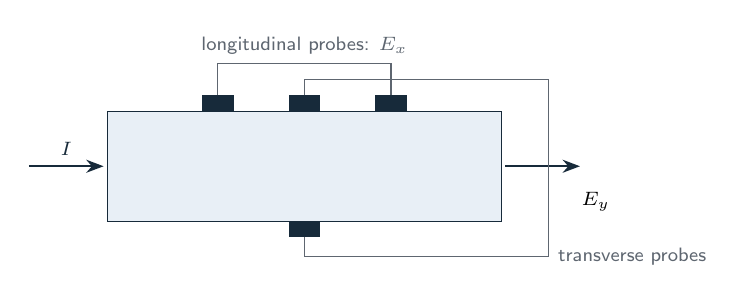
\begin{tikzpicture}[x=10mm,y=10mm]
\fill[colB!12,draw=ink] (0,0) rectangle (5,1.4);
\draw[->,ink,thick] (-1.0,0.7)--(-0.05,0.7) node[midway,above,font=\scriptsize]{$I$};
\draw[->,ink,thick] (5.05,0.7)--(6.0,0.7);
\fill[ink] (1.2,1.4) rectangle (1.6,1.6); \fill[ink] (3.4,1.4) rectangle (3.8,1.6);
\fill[ink] (2.3,-0.2) rectangle (2.7,0); \fill[ink] (2.3,1.4) rectangle (2.7,1.6);
\draw[rulegray] (1.4,1.6)--(1.4,2.0)--(3.6,2.0) node[midway,above,font=\scriptsize]{longitudinal probes: $E_x$}--(3.6,1.6);
\draw[rulegray] (2.5,-0.2)--(2.5,-0.45)--(5.6,-0.45) node[right,font=\scriptsize]{transverse probes};
\draw[rulegray] (2.5,1.6)--(2.5,1.8)--(5.6,1.8)--(5.6,-0.45);
\node[font=\scriptsize] at (6.2,0.25) {$E_y$};
\end{tikzpicture}
\figtext{A current $I$ flows along $x$. The two outer top contacts measure the longitudinal field $E_x$; the facing middle contacts (top and bottom) measure the transverse field $E_y$ at second order.}
\end{figpanel}

\question{C.3}{1.1}{\textbf{(a)} Show that $E_y/E_x^2=C_1\sigma+C_2$, and express $C_1$, $C_2$ through $A_1$, $A_2$, $\beta$.\par
\textbf{(b)} Three samples, which differ only in impurity density, give at low temperature (illustrative data):
\begin{center}\begin{tabular}{lccc}\toprule $\sigma$ (mS)&1.0&2.0&4.0\\ $E_y/E_x^2$ ($10^{-6}$ m/V)&0.9&1.3&2.1\\\bottomrule\end{tabular}\end{center}
Find $C_1$ and $C_2$ with units.\par
\textbf{(c)} Which mechanisms contribute to $C_1$, and which to $C_2$? Does $C_2$ measure the curvature dipole?\par
\textbf{(d)} Phonons are a second, time-dependent source of scattering. Explain why changing the temperature, instead of the impurity density, does not in general give the same straight line.}

\parttitle{D}{One broadening, many ensembles}{2.2}
The broadening of a level by collisions is $\Gamma=\hbar/(2\tau)$, the half-width it acquires when $i\Gamma$ is added to its energy.

\question{D.1}{0.8}{Consider three impurity ensembles with the same $n_i$: all impurities repulsive with $V_i=+V_0$; all attractive with $V_i=-V_0$; half of each, placed at random. \textbf{(a)} Find $\avg{V_i^2}$ and $\avg{V_i^3}$ for each. \textbf{(b)} Which of $1/\tau$, $\Gamma$, $\chi^{\rm cd}$, $\chi^{\rm sj}$, $\chi^{\rm isk}$, $\chi^{\rm esk}$ (extrinsic skew) are the same in all three ensembles, and which differ? \textbf{(c)} Is the second-order response determined by $\Gamma$ alone?}

Question D.2 concerns a different crystal: its clean part is inversion symmetric (no tilt), and disorder breaks inversion in every configuration. Each configuration $\mathcal C$ has an inverted partner $\mathcal I\mathcal C$, obtained by $\bm r\to-\bm r$, and $P[\mathcal I\mathcal C]=P[\mathcal C]$: the ensemble has inversion symmetry \emph{on average}. Assume that the steady current $\bm j_{\mathcal C}(\bm E)$ of each configuration is a well-defined function of its Hamiltonian and of $\bm E$.

\question{D.2}{0.9}{\textbf{(a)} Show that $\bm j_{\mathcal I\mathcal C}(-\bm E)=-\bm j_{\mathcal C}(\bm E)$, and hence that the averaged second-order coefficient vanishes, $\avg{\chi}=0$, although $\chi_{\mathcal C}\neq0$ in a typical configuration.\par
\textbf{(b)} A macroscopic sample consists of $M\gg1$ independent regions, and its measured $\chi$ is the average of their coefficients. How does the measured $\chi$ scale with $M$?\par
\textbf{(c)} Consider an open one-dimensional random chain whose ensemble has the same property, $P[\mathcal I\mathcal C]=P[\mathcal C]$, where inversion exchanges the two ends. It has two edge states, of energies $\epsilon_L(\mathcal C)$ at its left end and $\epsilon_R(\mathcal C)$ at its right end, with $\epsilon_L\neq\epsilon_R$ in a typical configuration. Show that $\epsilon_L$ and $\epsilon_R$ have the same probability distribution. Name the single property of the ensemble from which both (a) and (c) follow, and state how it constrains averaged quantities that inversion exchanges and averaged quantities that inversion reverses.}

\question{D.3}{0.5}{A low-frequency ($\omega\tau\ll1$) second-order Hall signal is measured in a time-reversal-symmetric crystal for several impurity densities. State what these data determine, what they cannot determine, and two further inputs that are needed to extract the Berry curvature dipole.}

%%%%%%%%%%%%%%%%%%%%%%%%%%%%%%%%%%%%%%%%%%%%%%%%%%%%%%%%%%%%%%%%%%%%%%%%%%%%%%%%%%%%%%%%%%%%%%%%
\problem{3}{Disorder in a two-cycle quantum pump}{10.0}

If the parameters of a lattice Hamiltonian are changed slowly and periodically, particles can be carried along the lattice, period after period, like goods on a conveyor belt (a \emph{Thouless pump}). For non-interacting fermions that fill a band separated by gaps from the other bands, the number of particles carried past any bond per period is an integer, the \emph{Chern number} of the band. For a clean chain it is computed from the Bloch states of the band as functions of the momentum $k$ and of the time $t$ in the cycle. A recent proposal uses repulsion to obtain a fraction.

Spinless fermions move on a chain of $5N$ sites with five sites per cell and $N$ particles (Fig.~\ref{fig:pump}). Set $\hbar=1$, count charge as a number of particles, and count transport to the right as positive. The Hamiltonian is
\[
H(t)=-\sum_j\big[J_j(t)c_{j+1}^\dagger c_j+\hc\big]+\sum_j\sum_{r=1}^{3}U_rn_jn_{j+r}+\sum_j\epsilon_jn_j,\qquad
J_j(t)=J+K\cos\Big(\frac{2\pi t}{T}+\frac{4\pi j}{5}\Big),
\]
with $K/J=-3/2$, repulsions $U_r\gg J$ between particles $r$ sites apart, and a period $T$ long compared with the inverse energy gaps of the relevant states (a slow cycle). Here $c_j$ removes a fermion from site $j$, $c_j^\dagger$ adds one, $n_j=c_j^\dagger c_j$, and ``h.c.'' is the Hermitian conjugate. Site $j=5R+\mu$ is orbital $\mu=0,\dots,4$ of cell $R$. The last term, a static random potential, is added here: the $\epsilon_j$ are independent and uniform on $[-W/2,W/2]$, and they do not change in time.

At strong repulsion and $W=0$, each particle occupies one of two localized orbitals per cell, built from the Bloch states of the two lowest bands (two-band \emph{Wannier orbitals}); the two orbital types are called \emph{flavors} $A$ and $B$ (Fig.~\ref{fig:flavors}). The orbitals of cell $R+1$ are those of cell $R$ shifted by five sites. If every particle follows its orbital as the parameters change, after one period it sits in an orbital of the other flavor, and after two periods it is back in its own flavor, one cell to the left. The charge carried per particle equals the displacement of its orbital centre in cells, so the charge per period, averaged over two periods, is $-1/2$. The flavor that a particle occupies at time $t$ after following its orbital from $t=0$ is called the \emph{followed} flavor. In short chains this works. In long chains, regions in which the particles occupy the other flavor (\emph{domains}) become energetically favourable during the cycle, and the fractional transport is expected to survive only for a finite \emph{prethermal lifetime}: the time over which a driven system keeps an ordered, non-equilibrium state before it heats up.

This problem asks: \emph{in a long chain with a static random potential, which quantity still defines the pumped charge, and how does the random potential change the protection of the fractional pump?} Part A first shows, in a simpler chain, that disorder can also create a topological edge state.

\begin{figpanel}{The driven chain}\label{fig:pump}
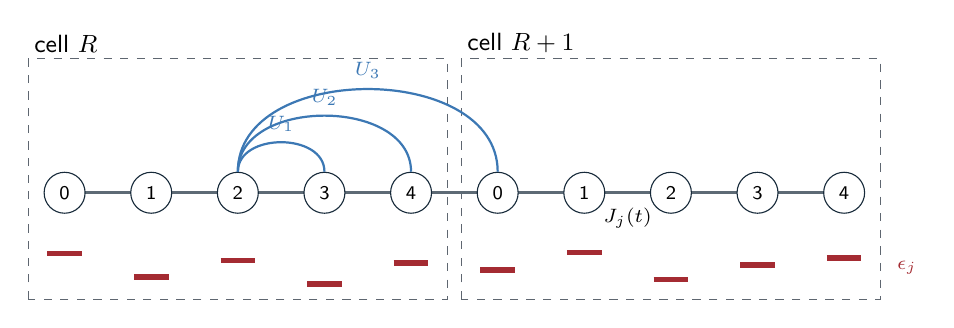
\begin{tikzpicture}[x=11mm,y=10mm]
\draw[dashed,rulegray] (-0.42,-1.35) rectangle (4.42,1.7);
\draw[dashed,rulegray] (4.58,-1.35) rectangle (9.42,1.7);
\node[font=\small,anchor=south west,inner sep=2pt] at (-0.42,1.7) {cell $R$};
\node[font=\small,anchor=south west,inner sep=2pt] at (4.58,1.7) {cell $R+1$};
\foreach \x in {0,...,8}{\draw[line width=1pt,ink!70] (\x,0)--(\x+1,0);}
\foreach \x in {0,...,9}{\pgfmathtruncatemacro{\s}{mod(\x,5)}\node[atom] (n\x) at (\x,0) {\s};}
\draw[colB,line width=0.8pt] (n2.north) .. controls +(0,0.5) and +(0,0.5) .. node[pos=0.5,above,font=\scriptsize]{$U_1$} (n3.north);
\draw[colB,line width=0.8pt] (n2.north) .. controls +(0,0.95) and +(0,0.95) .. node[pos=0.5,above,font=\scriptsize]{$U_2$} (n4.north);
\draw[colB,line width=0.8pt] (n2.north) .. controls +(0,1.4) and +(0,1.4) .. node[pos=0.5,above,font=\scriptsize]{$U_3$} (n5.north);
\node[font=\scriptsize] at (6.5,-0.32) {$J_j(t)$};
\foreach \x/\e in {0/0.3,1/-0.2,2/0.15,3/-0.35,4/0.1,5/-0.05,6/0.32,7/-0.25,8/0.05,9/0.2}{\draw[colR,line width=2pt] (\x-0.2,-0.95+\e*0.6)--(\x+0.2,-0.95+\e*0.6);}
\node[font=\scriptsize,text=colR,anchor=west] at (9.5,-0.95) {$\epsilon_j$};
\end{tikzpicture}
\figtext{Dashed boxes: two cells. Site $j=5R+\mu$ is orbital $\mu$ of cell $R$ (numbers in the circles). Black bonds: hoppings $J_j(t)$; blue arcs: repulsion $U_r$ between particles $r$ sites apart, drawn for one site only; red bars: the static random energies $\epsilon_j$ (schematic heights).}
\end{figpanel}

\smallheading{Useful information}
\begin{itemize}[leftmargin=6mm,itemsep=2pt,topsep=2pt]
\item Fermion operators obey $\{c_a,c_b^\dagger\}=\delta_{ab}$. For one particle, $-J_jc_{j+1}^\dagger c_j$ is the matrix element $-J_j$ from site $j$ to site $j+1$.
\item Heisenberg equation (with $\hbar=1$): $\dot O=i[H,O]$ for an operator without explicit time dependence. For fermions, $[c_a^\dagger c_b,n_j]=c_a^\dagger c_b(\delta_{bj}-\delta_{aj})$, and $n_in_l$ commutes with every $n_j$.
\item A variable uniform on $[-W/2,W/2]$ has mean $0$ and variance $W^2/12$. For random variables, $\Cov(x,y)=\avg{xy}-\avg x\,\avg y$; independent variables have zero covariance.
\item Law of large numbers: for independent, identically distributed $x_i$, $\frac1n\sum_{i=1}^n\ln|x_i|\to\avg{\ln|x|}$ as $n\to\infty$. Also $\int\ln x\,\dd x=x\ln x-x$, and $x\ln x\to0$ for $x\to0$.
\item A Hermitian $2\times2$ matrix can be written $M=h_0\id+h_xs_x+h_ys_y+h_zs_z$ with Pauli matrices $s_{x,y,z}$; then $h_z=(M_{11}-M_{22})/2$ and $h_x-ih_y=M_{12}$.
\item A sum of $\ell$ independent zero-mean Gaussian variables of variance $\sigma^2$ is Gaussian with variance $\ell\sigma^2$. Let $\Phi(z)$ be the probability that a standard Gaussian variable is below $z$: $\Phi(-1)=0.159$, $\Phi(-2)=0.0228$, $\Phi(-3)=0.00135$.
\item Independent rare events at a total rate $\Lambda$: the probability of no event during a time $t$ is $e^{-\Lambda t}$.
\end{itemize}

\parttitle{A}{Topology from disorder in a dimer chain}{1.6}
A particle hops on a long chain of cells, each with two sites $a_n$ and $b_n$ (Fig.~\ref{fig:dimer}):
\[
H_{\rm d}=\sum_{n}\Big[u_n\,a_n^\dagger b_n+v_n\,b_n^\dagger a_{n+1}+\hc\Big],
\]
with real, non-zero intracell hoppings $u_n$ and intercell hoppings $v_n$, and no on-site energies. The chain starts at the left with site $a_1$ and continues far to the right. For a regular chain ($u_n=u$, $v_n=v$) a state of energy zero localized at the left end (an \emph{edge state}) exists if and only if $|v|>|u|$; this is the topological phase of the chain. (On a finite chain the energy of such a state is exponentially small instead of zero.)

\begin{figpanel}{A dimer chain}\label{fig:dimer}
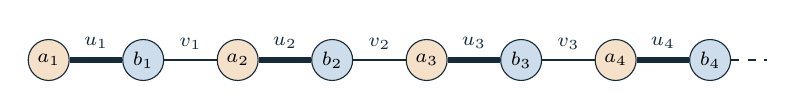
\begin{tikzpicture}[x=12mm,y=10mm]
\foreach \n in {1,...,4}{
 \node[atom,fill=colA!25] (a\n) at ({2*(\n-1)},0) {$a_{\n}$};
 \node[atom,fill=colB!25] (b\n) at ({2*(\n-1)+1},0) {$b_{\n}$};
 \draw[ink,line width=2pt] (a\n)--(b\n) node[midway,above,font=\scriptsize]{$u_{\n}$};}
\foreach \n [evaluate=\n as \m using int(\n+1)] in {1,...,3}{\draw[ink,line width=0.8pt] (b\n)--(a\m) node[midway,above,font=\scriptsize]{$v_{\n}$};}
\draw[ink,line width=0.8pt,dashed] (b4)--(7.6,0);
\end{tikzpicture}
\figtext{Intracell bonds $u_n$ (thick) and intercell bonds $v_n$ (thin). The chain starts with site $a_1$ and continues to the right (dashed).}
\end{figpanel}

\question{A.1}{0.8}{\textbf{(a)} Show that a state of energy zero with amplitudes only on the $a$ sites must satisfy $\psi(a_{n+1})=-(u_n/v_n)\,\psi(a_n)$.\par
\textbf{(b)} Let the pairs $(u_n,v_n)$ be independent and identically distributed. Show that, for large $n$, $\ln|\psi(a_n)/\psi(a_1)|\approx n\,\avg{\ln|u/v|}$. State the condition for a left edge state, and give the decay length of $|\psi|$ in cells.}

\question{A.2}{0.8}{Let $v_n=0.8$ for all $n$, and let $u_n$ be uniform on $[1-W/2,\,1+W/2]$ with $0\le W\le2$.\par
\textbf{(a)} Is the regular chain ($W=0$) in the topological phase? Find $\avg{\ln u}$ for $W=1$ and for $W=2$, and decide whether the edge state exists in each case. Give the decay length for $W=2$.\par
\textbf{(b)} Explain why the arithmetic mean $\avg u$ gives the wrong answer, and why the logarithmic mean decides.}

\parttitle{B}{Counting the pumped charge}{2.0}
Return to the pump Hamiltonian $H(t)$. Let $I_j$ be the operator of the particle current from site $j$ to site $j+1$, and $Q_j(t_{\rm i},t_{\rm f})=\int_{t_{\rm i}}^{t_{\rm f}}\langle I_j\rangle\dd t$ the charge carried across bond $j$ between the times $t_{\rm i}$ and $t_{\rm f}$.

\question{B.1}{1.0}{\textbf{(a)} Show that $I_j=i\big(J_jc_{j+1}^\dagger c_j-J_j^*c_j^\dagger c_{j+1}\big)$ satisfies $\dot n_j=I_{j-1}-I_j$, whatever the random energies $\epsilon_j$ and the repulsions $U_r$. (Here $J_j$ is real; the form with $J_j^*$ also holds for complex hoppings, which appear in B.2.)\par
\textbf{(b)} Show that the number of particles on the sites $j_1,\dots,j_2$ changes by $Q_{j_1-1}-Q_{j_2}$ between $t_{\rm i}$ and $t_{\rm f}$.\par
\textbf{(c)} A simulation of one disorder configuration on a long ring reports, for the window $[0,2T]$, the charges $Q_{10}=-1.00$, $Q_{30}=-0.99$, $Q_{50}=-0.62$, $Q_{70}=-1.01$. What happened on the sites $31,\dots,50$ and on the sites $51,\dots,70$? Can the transport of this configuration in this window be summarized by a single charge per period, the same for every bond?}

Close the chain into a ring of $L=5N$ sites and multiply the hopping of one bond by $e^{i\theta}$ (a magnetic flux $\theta$ through the ring; it changes no local property but shifts the allowed momenta of a clean ring). Use the following result: if the many-body ground state is unique and separated by an energy gap from all other states for all $t$ and all $\theta$, then, for a slow cycle, the charge carried across any bond in one period, averaged over $\theta\in[0,2\pi)$, is an integer $C$ (the \emph{many-body Chern number}).

\question{B.2}{1.0}{\textbf{(a)} Explain why this definition can be applied to each disorder configuration separately, and why it does not need a momentum $k$.\par
\textbf{(b)} In the two-cycle pump, the two lowest many-body states form a pair $\ket{\Psi_A}$, $\ket{\Psi_B}$ (all particles in flavor $A$, or all in $B$) that one period exchanges. Assume the following extension of the result: the pair is separated by a gap from all other states for all $t$ and $\theta$, and $q_1+q_2=C$ is an integer, where $q_1$ is the $\theta$-averaged charge carried in a period that starts in $\ket{\Psi_A}$ and $q_2$ in a period that starts in $\ket{\Psi_B}$. Show that the charge per period, averaged over two periods, is $C/2$ for either starting state. A calculation of orbital centres for this model gives displacements of $-0.582$ and $-0.418$ cells in two successive periods. Is this consistent with $C=-1$?\par
\textbf{(c)} Which assumption of (b) must hold uniformly in the chain length for the fractional value to be protected in a long chain?}

\parttitle{C}{What a random potential does to the flavors}{2.6}
Let $w_{R,A}(j)$ and $w_{R,B}(j)$ be the amplitudes on site $j$ of the two orthonormal flavor orbitals of cell $R$. Restricted to these two orbitals, the random potential $\sum_j\epsilon_jn_j$ acts on the particle of cell $R$ as the $2\times2$ matrix
\[
M^{(R)}_{\alpha\beta}=\sum_j\epsilon_j\,w_{R,\alpha}^*(j)\,w_{R,\beta}(j),\qquad\alpha,\beta\in\{A,B\},
\]
which defines $h_0^{(R)}$ and $\bm h^{(R)}=(h_x^{(R)},h_y^{(R)},h_z^{(R)})$ as in the Useful information (index 1 is $A$, index 2 is $B$). The component $h_z$ favours one flavor over the other (a \emph{flavor bias}); $h_x,h_y$ mix the two flavors. Write $d_{R}(j)=|w_{R,A}(j)|^2-|w_{R,B}(j)|^2$.

\question{C.1}{1.2}{\textbf{(a)} Express $h_z^{(R)}$ and $h_x^{(R)}-ih_y^{(R)}$ through the $\epsilon_j$ and the orbital amplitudes.\par
\textbf{(b)} Show that $\avg{h_z^{(R)}}=0$, $\Var h_z^{(R)}=\frac{W^2}{48}\sum_jd_R(j)^2$ and $\Cov\big(h_z^{(R)},h_z^{(R')}\big)=\frac{W^2}{48}\sum_jd_R(j)d_{R'}(j)$. When are the biases of two cells statistically independent?\par
\textbf{(c)} Consider two sites with $w_A=(\cos\phi,\sin\phi)$ and $w_B=(-\sin\phi,\cos\phi)$. Find $h_z$ and $h_x$ in terms of $\epsilon_1-\epsilon_2$ and $\phi$, and show that $h_x^2+h_z^2$ does not depend on $\phi$. What decides whether the same random potential acts as a bias or as a mixing?}

\begin{figpanel}{The two flavor orbitals of one cell}\label{fig:flavors}
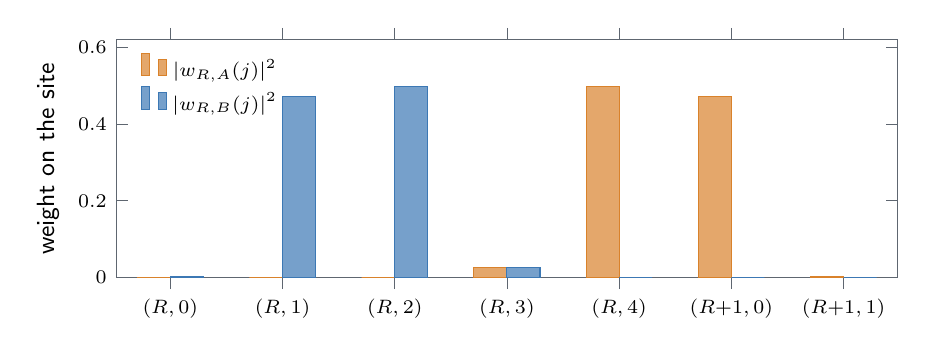
\begin{tikzpicture}
\begin{axis}[mbaxis,ybar=0pt,bar width=4.2mm,width=11.5cm,height=4.6cm,ymin=0,ymax=0.62,
  xtick={0,1,2,3,4,5,6},xticklabels={{$(R,0)$},{$(R,1)$},{$(R,2)$},{$(R,3)$},{$(R,4)$},{$(R{+}1,0)$},{$(R{+}1,1)$}},
  ylabel={weight on the site},legend style={at={(0.02,0.97)},anchor=north west},enlarge x limits=0.08]
\addplot[fill=colA!70,draw=colA] coordinates {(0,0.000) (1,0.000) (2,0.000) (3,0.027) (4,0.497) (5,0.472) (6,0.002)};
\addplot[fill=colB!70,draw=colB] coordinates {(0,0.002) (1,0.472) (2,0.497) (3,0.027) (4,0.000) (5,0.000) (6,0.000)};
\legend{$|w_{R,A}(j)|^2$,$|w_{R,B}(j)|^2$}
\end{axis}
\end{tikzpicture}
\figtext{Computed for the clean single-particle chain at $K/J=-3/2$ and $t=0$: site weights of the two flavor orbitals of cell $R$. Sites are labelled (cell, orbital). The centre of the $A$ orbital lies $0.89$ cells, that of the $B$ orbital $0.31$ cells, to the right of site $(R,0)$. At $t=0$ the followed flavor is $A$. The very small bars on $(R,0)$ and $(R{+}1,1)$ are tails. Single-particle geometry only.}
\end{figpanel}

For the orbitals of Fig.~\ref{fig:flavors}, use the rounded weights
\begin{center}\small\begin{tabular}{lccccc}\toprule
site&$(R,1)$&$(R,2)$&$(R,3)$&$(R,4)$&$(R{+}1,0)$\\\midrule
$|w_{R,A}|^2$&0&0&0.03&0.50&0.47\\
$|w_{R,B}|^2$&0.47&0.50&0.03&0&0\\\bottomrule
\end{tabular}\end{center}
and neglect all other sites (weights below 0.003 are rounded to 0). The products $w_{R,A}^*(j)w_{R,B}(j)$, which involve the small tails, are real; they are non-zero only on the sites $(R,1)$, $(R,3)$, $(R{+}1,0)$, where they equal $-0.013$, $+0.027$, $-0.013$.

\question{C.2}{0.8}{\textbf{(a)} Find $\sum_jd_R(j)^2$ and the rms flavor bias $h_z$ in units of $W$.\par
\textbf{(b)} Find the rms flavor mixing $h_x$ in units of $W$. Which effect of the random potential dominates for these orbitals?\par
\textbf{(c)} In this approximation, are the biases of neighbouring cells correlated?}

The random potential does not change in time, and $H(t+T)=H(t)$, so the set of flavor orbitals at $t+T$ is the same as at $t$. A particle that occupies an $A$ orbital at time $t$ occupies a $B$ orbital at time $t+T$.

\question{C.3}{0.6}{Let $g^{\rm f}_R(t)$ (f for ``followed'') be the energy released by the random potential, through the bias $h_z$ only, when the particle of cell $R$ moves from its followed orbital to the other orbital of the cell: $g^{\rm f}_R>0$ if the move lowers the energy. Show that $g^{\rm f}_R(t+T)=-g^{\rm f}_R(t)$ (the cell label may shift by one, because the followed particle has moved by part of a cell). What does this imply for an estimate of domain energies made at one instant of the cycle?}

\parttitle{D}{Domains in a long disordered chain}{3.8}
At strong repulsion, describe the chain by one variable per cell: $\eta_R=+1$ if the particle of cell $R$ is in the followed flavor, $\eta_R=-1$ if it is in the other one. Turning a block $D$ of $\ell$ consecutive cells to $\eta=-1$ (a domain, Fig.~\ref{fig:domain}) changes the energy by
\[
\Delta E_D(t)=E_{\rm w}-2\sum_{R\in D}\big[\beta(t)+h_R(t)\big],
\]
where $E_{\rm w}>0$ is the cost of the two domain walls, $h_R=g^{\rm f}_R/2$ is the random bias of Part C, and $\beta(t)$ is the bias of the clean chain, with $\beta>0$ favouring the other flavor. By the argument of C.3, $\beta(t+T)=-\beta(t)$, so $\beta$ changes sign during each period and vanishes at some instants; its maximum is $\beta_{\max}>0$. In the clean chain, the rate of creating a domain of $\ell$ cells decreases roughly exponentially with $\ell$, because all $\ell$ particles must change orbital together. Use $E_{\rm w}=0.4J$ and $\beta_{\max}=0.01J$.

\begin{figpanel}{A domain}\label{fig:domain}
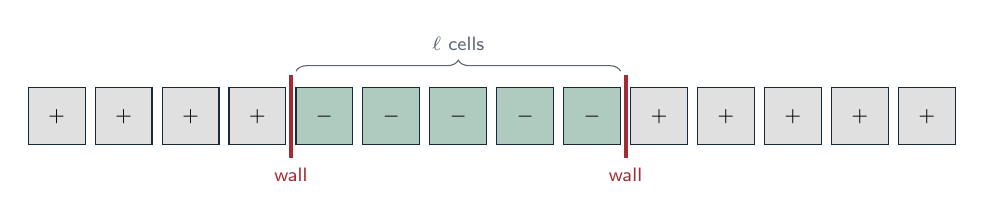
\begin{tikzpicture}[x=8.5mm,y=8.5mm]
\foreach \x in {0,...,13}{%
  \ifnum\x>3 \ifnum\x<9
    \fill[colG!35,draw=ink] (\x,0) rectangle (\x+0.85,0.85); \node[font=\scriptsize] at (\x+0.425,0.425) {$-$};
  \else
    \fill[black!12,draw=ink] (\x,0) rectangle (\x+0.85,0.85); \node[font=\scriptsize] at (\x+0.425,0.425) {$+$};
  \fi\else
    \fill[black!12,draw=ink] (\x,0) rectangle (\x+0.85,0.85); \node[font=\scriptsize] at (\x+0.425,0.425) {$+$};
  \fi}
\draw[colR,line width=1.4pt] (3.925,-0.2)--(3.925,1.05);
\draw[colR,line width=1.4pt] (8.925,-0.2)--(8.925,1.05);
\draw[decorate,decoration={brace,amplitude=4pt},rulegray] (4,1.1)--(8.85,1.1) node[midway,above=4pt,font=\scriptsize]{$\ell$ cells};
\node[font=\scriptsize,text=colR] at (3.925,-0.45) {wall};
\node[font=\scriptsize,text=colR] at (8.925,-0.45) {wall};
\end{tikzpicture}
\figtext{Grey ($\eta=+1$): cells in the followed flavor. Green ($\eta=-1$): a domain of $\ell$ cells in the other flavor, bounded by two walls (red). The colours mean followed/other, not $A$/$B$.}
\end{figpanel}

\question{D.1}{0.6}{In the clean chain ($h_R=0$), find the smallest number of cells $\ell$ for which a domain strictly lowers the energy ($\Delta E_D<0$) at $\beta=\beta_{\max}$. Why does a long clean chain still keep its order for a long time?}

Now take an instant with $\beta=0$, and treat the $h_R$ as independent zero-mean Gaussian variables of rms $\sigma_h$ (each is a sum of several site energies).

\question{D.2}{1.2}{\textbf{(a)} Find the probability $p(\ell)$ that a given block of $\ell$ cells has $\Delta E_D<0$, and the length $\ell$ at which $p=\Phi(-1)$, in terms of $E_{\rm w}/\sigma_h$.\par
\textbf{(b)} Take $\sigma_h=0.05J$. Find the random-potential width $W$ that gives this $\sigma_h$ for the orbitals of C.2. Find $p(4)$ and estimate how many of the $2500$ disjoint blocks of 4 cells in a ring of $N=10^4$ cells have $\Delta E_D<0$.\par
\textbf{(c)} Explain why, for any $\sigma_h>0$, a long enough chain contains blocks with $\Delta E_D<0$ even at $\beta=0$, whereas the clean chain at $\beta=0$ contains none. What does this imply for a gap that is uniform in the chain length?}

Suppose that \emph{defects} --- regions in which the pump has stopped working, for example heated regions left behind by domains --- start independently in each cell at a rate $\gamma$ per period, and that each defect then occupies a fixed region of $\xi$ cells without spreading; overlaps of defects can be neglected. The \emph{ring-averaged} charge per period is the charge per period averaged over all bonds of the ring.

\question{D.3}{1.0}{\textbf{(a)} Find the time $t_{\rm first}$, in periods, at which the probability of at least one defect in the ring reaches $1-1/e$, and the time $t_\kappa$ at which the ring-averaged charge per period has dropped by a fraction $\kappa\ll1$.\par
\textbf{(b)} Evaluate $t_{\rm first}$ and $t_\kappa$ for $N=10^4$, $\gamma=10^{-6}$, $\xi=10$, $\kappa=0.01$.\par
\textbf{(c)} Which of the two times depends on $N$? Which one is the lifetime of the pump in a large system? How does $t_\kappa$ change if each defect spreads by $s_{\rm d}$ cells per period on each side?}

\question{D.4}{1.0}{A prediction of the lifetime of the disordered fractional pump in a long chain still needs four inputs that this problem has not computed: one about the random fields, one about the creation of domains, one about the motion of domain walls, and one about the measured charge. State each input. Explain why neither the many-body Chern number of B.2 nor the domain energy $\Delta E_D$ at one instant gives this lifetime.}

\vfill
\begin{center}\textbf{End of the theoretical examination}\end{center}
\end{document}
